\documentclass{standalone}
\usepackage{amsmath}
\usepackage{graphicx}
\usepackage{tikz}
\usetikzlibrary{shapes,positioning,arrows,automata}
\usepackage{graphicx}
\usepackage{parskip}
\usepackage{amsthm}
\usepackage{mathtools}
\usepackage[utf8]{inputenc}
\usepackage{longfbox}
\begin{document}
\lfbox[border-width=0pt,background-color=white]{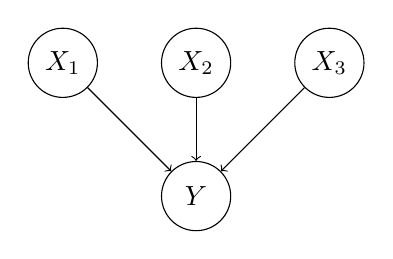
\begin{tikzpicture}[node distance=2cm and 2cm]
\node[state] (w1) {$X_1$};
\node[state] (w2) [right=8mm of w1] {$X_2$};
\node[state] (w3) [right=8mm of w2] {$X_3$};
\node[state] (v1) [below =8mm of w2] {$Y$};
\path[->] (w1) edge node[label] {} (v1);
\path[->] (w2) edge node[label] {} (v1);
\path[->] (w3) edge node[label] {} (v1);\end{tikzpicture}}
\end{document}
